\documentclass{oci}
\usepackage[utf8]{inputenc}
\usepackage{lipsum}
\usepackage{subcaption}

\title{La leyenda de Zolda}

\begin{document}
\begin{problemDescription}
  \emph{La leyenda de Zolda} es una popular saga de videojuegos con ya más de 19
  títulos, incluyendo aclamadas entregas como \emph{La zampoña del tiempo},
  \emph{La princesa del amanecer}, \emph{Un enlace al futuro} y \emph{Aliento de
  la civilización}.

  En la última versión del videojuego, disponible solo desde hace algunos días,
  existe una modalidad donde el personaje principal, \emph{Lonk}, debe
  enfrentarse a una horda de \emph{meblins}.
  En esta modalidad el escenario corresponde a un plano cartesiano y nuestro
  héroe se encontrará siempre en la coordenada $(0,0)$, mientras que los meblins
  pueden estar en cualquier coordenada distinta a esta.

  Como los fans encontraron la última versión demasiado, fácil los
  desarrolladores decidieron hacer esta versión mucho más difícil.
  Para esto decidieron aumentar la cantidad de meblins.
  En esta versión habrá tantos meblins que es más sencillo describir las
  posiciones donde NO hay meblins.

  En la siguiente figura Lonk está representado con una estrella y los meblins
  mediante puntos.
  Adicionalmente están marcados con un cuadrado los puntos que no contienen meblins.
  Como puede apreciarse hay 5 puntos que no contienen meblins: $(-1,0)$, $(-1,-2)$,
  $(1,1)$, $(3,3)$ y $(3, -3)$.
  \begin{center}
  \includegraphics{zolda}
  \end{center}
  Para pasar de nivel, Lonk debe eliminar al menos $K$ meblins del escenario
  usando su poderoso \emph{ataque de giro}.
  Con este ataque Lonk puede dañar todo a su alrededor de un solo golpe.
  Dependiendo la potencia que use, Lonk puede variar el radio de alcance de su
  ataque.
  Específicamente, si Lonk escoge un radio entero $R$ eliminará a todos los
  meblins que se encuentren dentro de este radio.
  Con el fin de reservar energía para el futuro una buena estrategia es siempre
  utilizar el menor radio con el cuál es posible eliminar a los $K$ meblins.
  Por ejemplo, en el escenario mostrado anteriormente, si el objetivo es eliminar
  $K=4$ meblins, el menor radio con que esto es posible es 2.

  \begin{figure}[h]
    \centering
    \begin{subfigure}{0.3\textwidth}
      \centering
      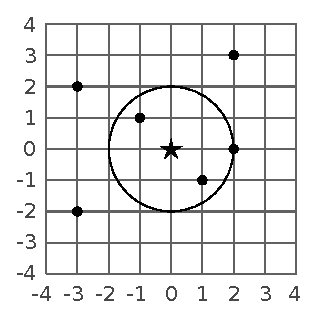
\includegraphics[scale=0.8]{zolda2}
      \caption*{Con $R=1$ Lonk elimina solo 3 meblins.}
    \end{subfigure}
    \hspace{3em}
    \begin{subfigure}{0.3\textwidth}
      \centering
      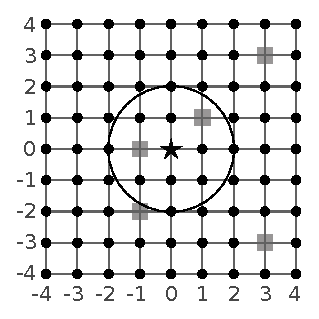
\includegraphics[scale=0.8]{zolda3}
      \caption*{Con $R=2$ Lonk elimina 10 meblins.}
    \end{subfigure}
  \end{figure}

\end{problemDescription}

\newpage
\begin{inputDescription}
  La entrada está descrita en varias líneas.
  La primera línea contiene dos enteros $N$ y $K$ correspondientes
  respectivamente a la cantidad de posiciones donde NO hay meblins y la cantidad
  de meblins que hay que eliminar para pasar de nivel.
  A continuación se entregan $N$ líneas cada una conteniendo dos enteros $X_i$ y
  $Y_i$ que representan las coordenadas de un punto donde no hay un meblin
  ($10^{-9}\leq X_i, Y_i\leq 10^9$).
  Se garantiza que todas estas líneas serán distintas.
  Notar que el punto $(0, 0)$ nunca aparecerá en la lista, pero esta posición nunca
  contendrá un meblin pues es la posición donde se encuentra Lonk.
\end{inputDescription}

\begin{outputDescription}
  La salida debe ser un único entero correspondiente al radio $R$
  mínimo con el cual Lonk puede eliminar $K$ meblins.
\end{outputDescription}

\begin{scoreDescription}
\score{5} Se probarán varios casos donde $N=0$ y $0 < K \leq 10$.
\score{10} Se probarán varios casos donde $0 < N \leq 10$ y $0 < K \leq 10$.
\score{30} Se probarán varios casos donde $0 \leq N \leq 100$ y $10 < K \leq 5000$.
\score{55} Se probarán varios casos donde $0 \leq N \leq 10^5$ y $1000 < K \leq 10^{10}$.
\end{scoreDescription}

\begin{sampleDescription}
\sampleIO{sample-1}
\end{sampleDescription}

\end{document}
